\documentclass[11pt, a4paper]{article}
\usepackage[a4paper, margin=2.5cm]{geometry}
\usepackage[T1]{fontenc}
\usepackage[utf8]{inputenc}
\usepackage{lmodern}
\usepackage[portuguese]{babel}
\renewcommand{\familydefault}{\sfdefault}
\usepackage{booktabs}
\usepackage{amsmath}
\usepackage{longtable}
\usepackage{graphicx}
\usepackage{float}
\usepackage[hidelinks]{hyperref}

% Figuras e tabela geradas pelos scripts de src/scripts/ (rodar a partir da raiz do repositório).
% Em editores online (Prism, Overleaf) não existe ../data: envie os arquivos de data/
% (grafico_*.pdf e tabela_ganho.tex) para uma pasta figuras/ ao lado deste .tex.
% Localmente, os arquivos são lidos direto de ../data/.
\graphicspath{{figuras/}{../data/}}

\title{Segundo Exercício-Programa\\ \large Sistemas Operacionais}
\author{
    Manuela Campos de Amorim (Nº USP: 16887191) \\
    {[Membro 2]} (Nº USP: [Inserir]) \\
    {[Membro 3]} (Nº USP: [Inserir]) \\
    Sabrina Cristan (Nº USP: 16837632)
}
\date{Novembro de 2026}

\begin{document}

\maketitle

\begin{abstract}
    [Espaço reservado para o resumo do relatório. Aqui vocês devem escrever um parágrafo condensando o objetivo do experimento (comparar o tempo de acesso concorrente à base de dados em RAM) e a conclusão geral obtida sobre qual abordagem foi melhor e em qual cenário.]
\end{abstract}

\section{Introdução}
[Espaço reservado para a introdução. Apresentar o problema de Leitores e Escritores, o cenário proposto pelo EP (acessos concorrentes a um texto filosófico na memória) e o que se espera observar ao testar diferentes proporções de threads.]

\section{Metodologia do experimento}
\subsection{Base de dados e região crítica}
% Detalhes de implementação que podem ajudar a escrever esta seção:
% - Base: String[] com as 36.242 palavras do bd.txt, carregada uma vez; escritas ficam só em RAM.
% - Threads: 100 acessos aleatórios (ThreadLocalRandom) + sleep(1) dentro da região crítica.
% - Travas: as duas usam monitor Java (synchronized + wait/notifyAll), para comparar a política
%   e não primitivas diferentes. L/E: escritor espera se houver escritor ativo, leitor ativo
%   OU leitor esperando (prioridade de leitura também na saída de um escritor).
% - Orquestração: a cada rodada, trava nova e 100 threads criadas com new e colocadas em
%   posições ainda vazias sorteadas do arranjo. Cronômetro (System.nanoTime) dispara com todas
%   em NEW e para após join() da última. 101 proporções x 50 repetições x 2 travas = 10.100 rodadas.
% - Tempos guardados em memória e gravados no CSV só no final (sem I/O durante a medição).
% - 20 rodadas de aquecimento do JIT descartadas; em cada repetição as duas travas rodam em
%   sequência, alternando qual vai primeiro.
% - Ambiente: Intel Core i7-1185G7 (4 núcleos / 8 threads), 30 GB de RAM, Ubuntu 24.04,
%   OpenJDK 21.0.13; experimento completo levou 866 s (~14,4 min).

\section{Resultados e análise de desempenho}
\label{sec:resultados}

Esta seção apresenta os tempos medidos nas 10.100 rodadas do experimento (101 proporções
$\times$ 50 repetições $\times$ 2 travas). Cada ponto discutido é a média das 50 repetições
de uma proporção. A tabela completa, com as 101 proporções, está na
Tabela~\ref{tab:ganho}, no apêndice.

\subsection{Comparação de médias gerais}
\label{sec:medias}

A Figura~\ref{fig:desempenho} mostra o tempo médio de execução das duas implementações em
função da proporção de leitoras. Os dois comportamentos são bem diferentes.

\begin{itemize}
    \item \textbf{Trava global:} o tempo fica praticamente constante, em torno de
    \textbf{111,7\,ms} (entre 110,9 e 116,5\,ms), qualquer que seja a proporção. Como só uma
    \textit{thread} entra na base por vez, as 100 \textit{threads} passam uma a uma pela região
    crítica. Cada uma a ocupa pelo tempo da soneca de 1\,ms (que, na prática, dura cerca de
    1,1\,ms por causa da latência para o escalonador acordar a \textit{thread}) mais os 100
    acessos à memória, que custam frações de microssegundo. Assim,
    $T_{\text{global}} \approx 100 \times 1{,}1\,\text{ms}$, e não importa se quem está dentro
    lê ou escreve.

    \item \textbf{Leitores e Escritores:} o tempo cai de forma praticamente linear conforme
    aumentam as leitoras, de 112,5\,ms (0 leitoras) até 4,2\,ms (100 leitoras). Uma regressão
    linear sobre as 101 médias dá
    \[
        T_{\text{L/E}} \approx 1{,}12 \cdot E + 3{,}8\ \text{ms} \qquad (R^2 = 0{,}999),
    \]
    em que $E$ é o número de escritoras. O coeficiente angular (1,12\,ms) é exatamente o custo
    de uma passagem exclusiva pela região crítica, o mesmo da trava global: \textbf{cada
    escritora continua sendo serializada}, enquanto as leitoras dormem juntas e somam, em
    conjunto, o equivalente a poucas passagens (o termo constante de 3,8\,ms).
\end{itemize}

\begin{figure}[H]
    \centering
    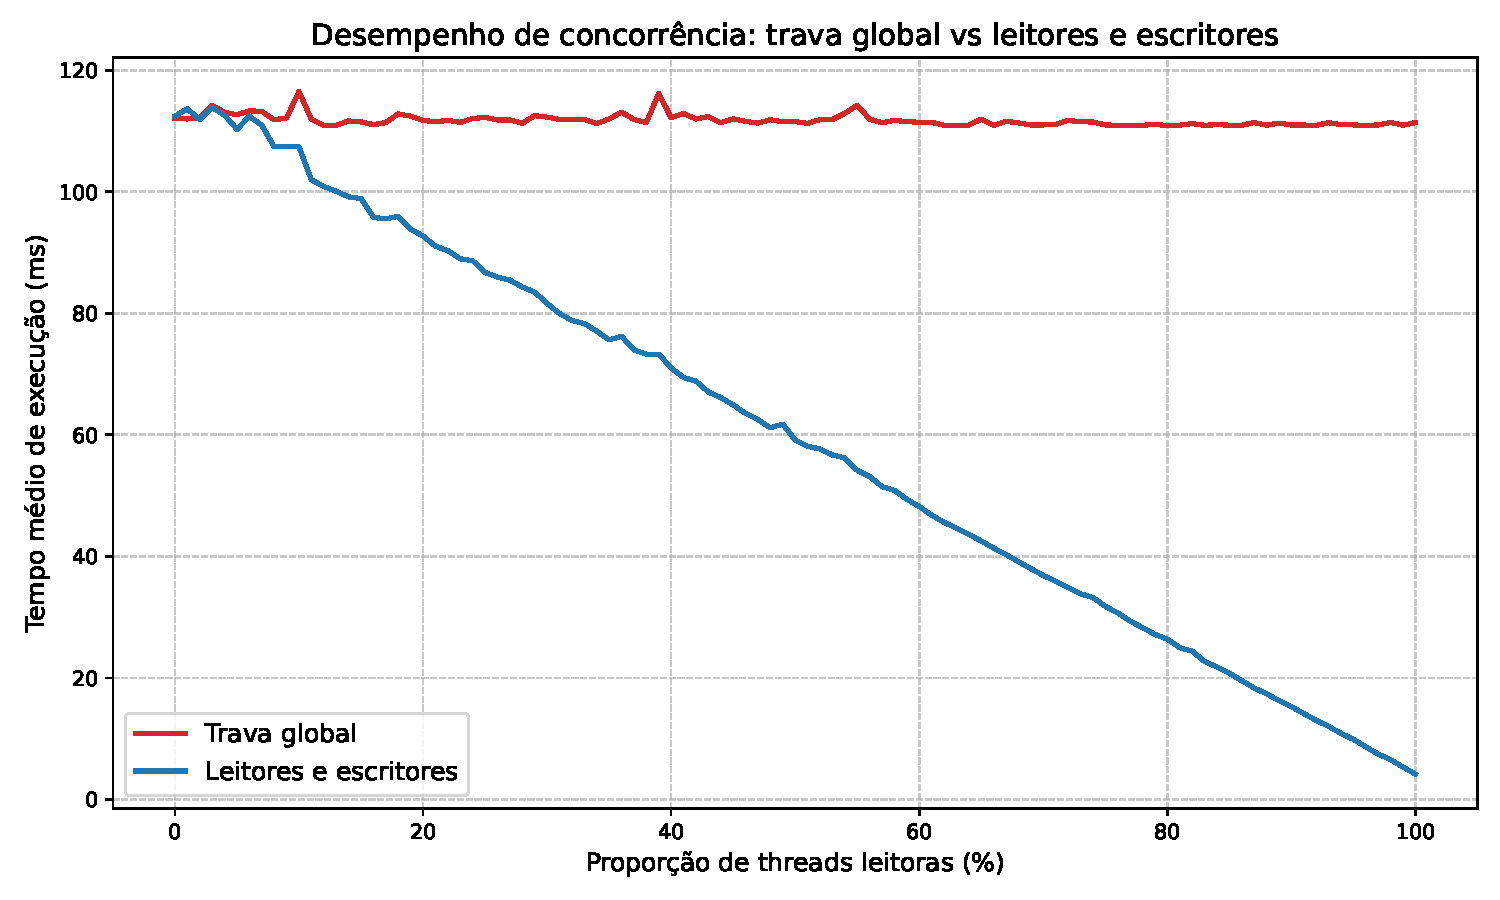
\includegraphics[width=0.9\textwidth]{grafico_desempenho.pdf}
    \caption{Tempo médio de execução (50 repetições) por proporção de threads leitoras.}
    \label{fig:desempenho}
\end{figure}

Ou seja, o ganho de Leitores e Escritores vem de permitir que as leitoras compartilhem a
soneca de 1\,ms. Esse é justamente o trecho mais caro da região crítica, já que os 100
acessos à memória são desprezíveis perto dele. Com a trava global, 100 leitoras custam 100
sonecas em sequência. Com Leitores e Escritores, custam praticamente uma.

\subsection{Variância e efeito do escalonador}
\label{sec:variancia}

A Figura~\ref{fig:desvio} mostra a média de cada proporção com uma faixa de um desvio padrão,
e a Figura~\ref{fig:boxplots} mostra a distribuição das 50 repetições para 10\%, 50\% e 90\%
de leitoras.

\begin{figure}[H]
    \centering
    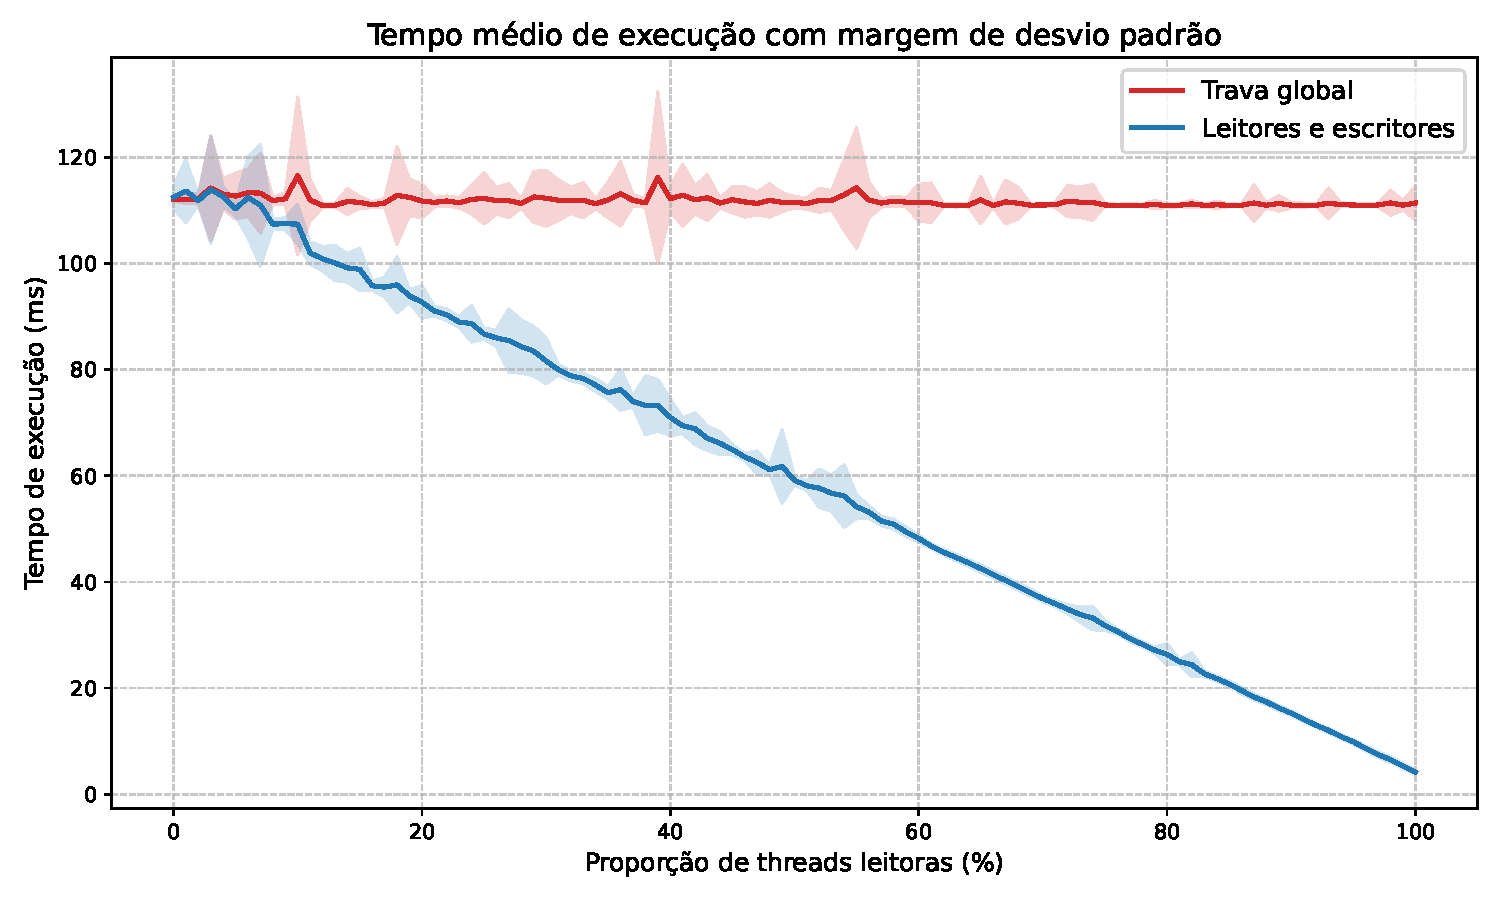
\includegraphics[width=0.85\textwidth]{grafico_desvio_padrao.pdf}
    \caption{Tempo médio com faixa de $\pm$ um desvio padrão.}
    \label{fig:desvio}
\end{figure}

\begin{figure}[H]
    \centering
    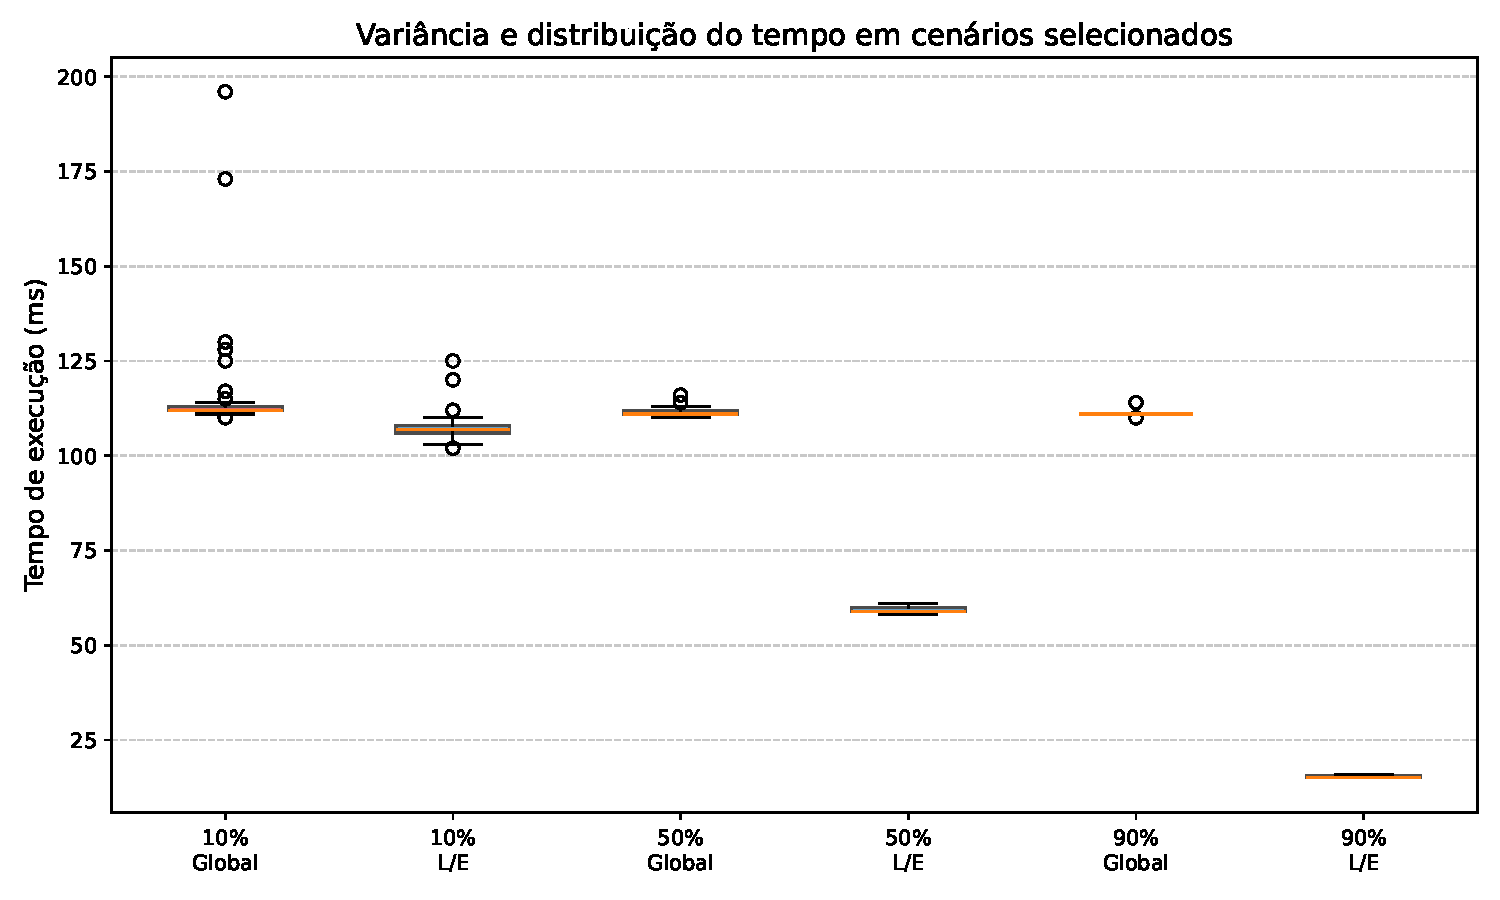
\includegraphics[width=0.85\textwidth]{grafico_boxplots.pdf}
    \caption{Distribuição das 50 repetições em cenários selecionados.}
    \label{fig:boxplots}
\end{figure}

A dispersão é pequena nas duas implementações: o desvio padrão médio entre as proporções foi de
2,5\,ms para a trava global e 2,0\,ms para Leitores e Escritores. Na maior parte das
repetições, a variação fica abaixo de 1\,ms. Isso confirma que a soneca de 1\,ms domina o
tempo e mascara o ruído da medição, como antecipado no enunciado.

As exceções são \textit{outliers} isolados, causados pelo escalonador do sistema operacional:
rodadas em que alguma \textit{thread} demorou a ser acordada ou perdeu a CPU para outro processo
da máquina. O caso mais visível é o de 10\% de leitoras com trava global
(Figura~\ref{fig:boxplots}), em que duas repetições levaram 173 e 196\,ms contra uma mediana de
112\,ms. Elas sozinhas puxam a média dessa proporção para 116,5\,ms e explicam o pico isolado na
curva da trava global. Por isso a mediana é uma boa referência complementar à média: em 10\%,
ela vale 112\,ms (global) contra 107\,ms (L/E).

Os \textit{outliers} afetam as duas travas, porque dependem do escalonador e não da política de
acesso. Na trava global, porém, um atraso de uma \textit{thread} atrasa diretamente todas as que
estão na fila. Em Leitores e Escritores, um atraso de uma leitora pode ser escondido pelas
outras leitoras que estão na base ao mesmo tempo.

\subsection{Custo computacional e pior cenário}
\label{sec:pior}

O pior cenário para Leitores e Escritores é aquele em que não há nenhuma leitora para
aproveitar o acesso compartilhado: 0 leitoras e 100 escritoras (Figura~\ref{fig:pior}). Nesse
caso as duas soluções fazem exatamente o mesmo trabalho (exclusão mútua entre escritoras), e a
única diferença é o custo extra de manter os contadores de leitoras ativas e em espera.

\begin{figure}[H]
    \centering
    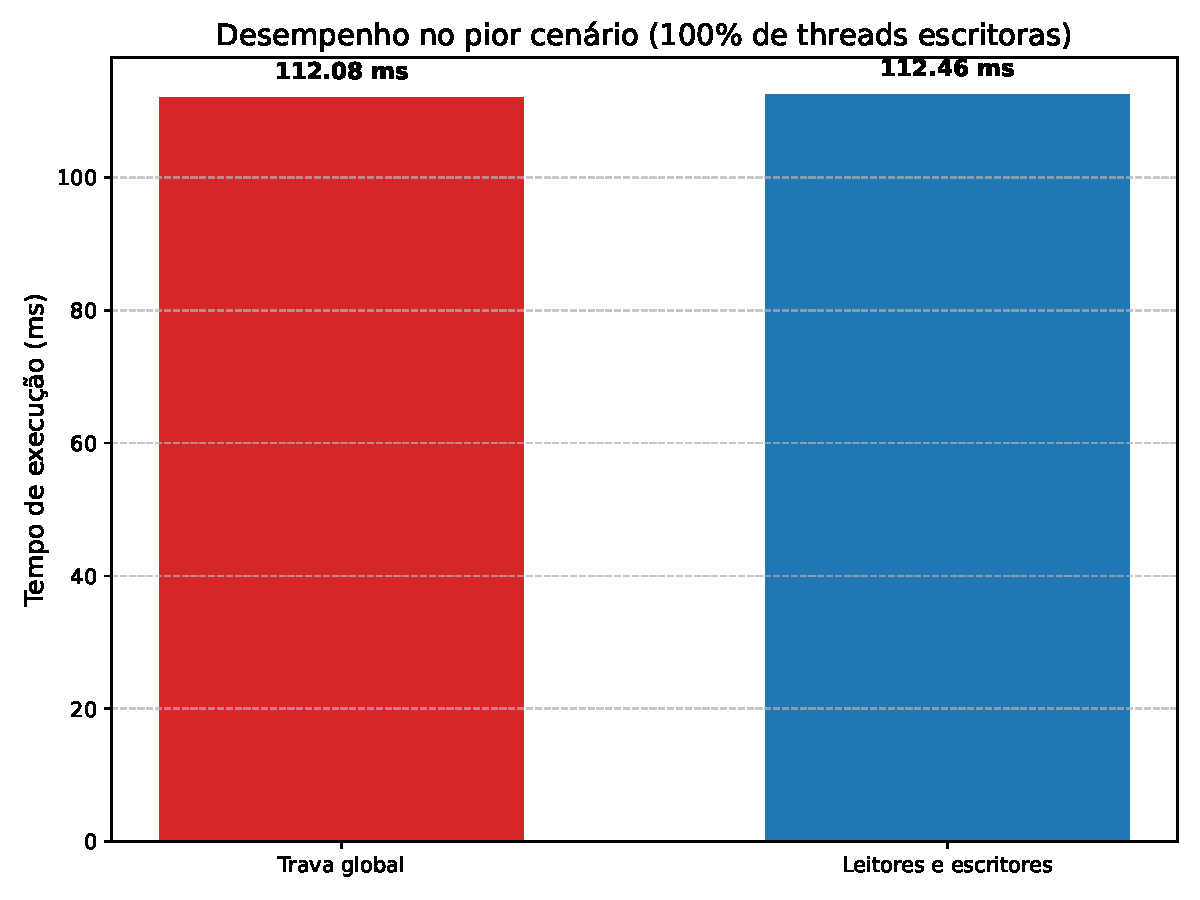
\includegraphics[width=0.65\textwidth]{grafico_pior_cenario.pdf}
    \caption{Tempo médio com 0 leitoras e 100 escritoras.}
    \label{fig:pior}
\end{figure}

O resultado foi 112,08\,ms para a trava global e 112,46\,ms para Leitores e Escritores, uma
diferença de 0,34\%. Com 1 leitora e 99 escritoras, a diferença foi de 1,48\% (111,98 contra
113,64\,ms), mas o desvio padrão de L/E nesse cenário (5,98\,ms) é maior que a própria
diferença. Na prática, os dois casos são um empate: o \textit{overhead} da política de
prioridade (alguns acessos a inteiros dentro do monitor) é desprezível perto de 1\,ms de
soneca. As duas travas usam a mesma primitiva (monitor Java com \texttt{wait}/\texttt{notifyAll}),
então não há custo de primitiva que favoreça uma delas.

Vale notar também que a inanição de escritoras, possível com a prioridade para leitoras, não
apareceu como aumento do tempo total. Cada leitora sai da base depois de 100 acessos e
1\,ms, então a fila de leitoras sempre se esvazia e as escritoras acabam entrando. A inanição
afeta a espera de cada escritora individualmente, mas não o tempo até a última
\textit{thread} terminar, que é o que foi medido.

\subsection{Ponto de virada}
\label{sec:virada}

A Tabela~\ref{tab:resumo} resume o ganho percentual de Leitores e Escritores sobre a trava
global, calculado como
$\text{ganho} = (T_{\text{global}} - T_{\text{L/E}}) / T_{\text{global}} \times 100$.
Valores positivos indicam que Leitores e Escritores foi mais rápido.

\begin{table}[H]
    \centering
    \caption{Ganho de Leitores e Escritores em proporções selecionadas (média de 50 repetições).}
    \label{tab:resumo}
    \begin{tabular}{rrrrr}
        \toprule
        Leitoras & Escritoras & Trava global (ms) & L/E (ms) & Ganho (\%) \\
        \midrule
          0 & 100 & 112,08 & 112,46 & $-$0,34 \\
          1 &  99 & 111,98 & 113,64 & $-$1,48 \\
          2 &  98 & 112,24 & 111,86 &    0,34 \\
          5 &  95 & 112,68 & 110,28 &    2,13 \\
         10 &  90 & 116,48 & 107,40 &    7,80 \\
         25 &  75 & 112,24 &  86,72 &   22,74 \\
         50 &  50 & 111,54 &  59,14 &   46,98 \\
         75 &  25 & 111,00 &  31,78 &   71,37 \\
         90 &  10 & 110,98 &  15,26 &   86,25 \\
         99 &   1 & 110,96 &   5,32 &   95,21 \\
        100 &   0 & 111,38 &   4,16 &   96,27 \\
        \bottomrule
    \end{tabular}
\end{table}

\textbf{Houve ganho com Leitores e Escritores a partir de 2 leitoras}, e ele cresce de forma
contínua com a proporção de leitoras. Só nas proporções de 0 e 1 leitora a trava global foi
marginalmente mais rápida, dentro da margem de ruído. Com poucas leitoras (2 a 9) o ganho
ainda é pequeno (até cerca de 5\%) e da ordem da variação entre repetições. A partir de
\textbf{10 leitoras} ele passa de 5\% e se torna claramente significativo. Com 50\% de
leitoras, L/E já leva menos da metade do tempo da trava global, e com 100 leitoras o ganho
chega a \textbf{96\%} (4,2 contra 111,4\,ms, cerca de 27 vezes mais rápido).

Pelo modelo linear da Seção~\ref{sec:medias}, o ganho esperado é aproximadamente proporcional
ao número de leitoras: cada leitora deixa de pagar uma passagem exclusiva de cerca de 1,1\,ms.
Por isso não existe propriamente um ``custo de gerenciar prioridades'' que precise ser pago
antes de o ganho aparecer. Leitores e Escritores nunca é pior que a trava global de forma
significativa e passa a ser melhor assim que existem leitoras suficientes para compartilhar a
base.

\section{Conclusão}
[Espaço reservado para a conclusão final do relatório. Sintetizar se e quando houve ganho com a solução de Leitores e Escritores, amarrando os dados com a teoria de Sistemas Operacionais.]

\appendix
\section{Tempos médios por proporção}
\InputIfFileExists{figuras/tabela_ganho.tex}{}{\begin{longtable}{rrrr}
\caption{Tempo médio (50 repetições) por proporção de leitoras e ganho da solução de leitores e escritores sobre a trava global.} \label{tab:ganho} \\
\toprule
Proporção de leitoras (\%) & Trava global (ms) & Leitores e escritores (ms) & Ganho percentual (\%) \\
\midrule
\endfirsthead
\caption[]{Tempo médio (50 repetições) por proporção de leitoras e ganho da solução de leitores e escritores sobre a trava global.} \\
\toprule
Proporção de leitoras (\%) & Trava global (ms) & Leitores e escritores (ms) & Ganho percentual (\%) \\
\midrule
\endhead
\midrule
\multicolumn{4}{r}{Continua na próxima página} \\
\midrule
\endfoot
\bottomrule
\endlastfoot
0 & 112.08 & 112.46 & -0.34 \\
1 & 111.98 & 113.64 & -1.48 \\
2 & 112.24 & 111.86 & 0.34 \\
3 & 114.20 & 113.88 & 0.28 \\
4 & 113.08 & 112.60 & 0.42 \\
5 & 112.68 & 110.28 & 2.13 \\
6 & 113.32 & 112.42 & 0.79 \\
7 & 113.24 & 110.94 & 2.03 \\
8 & 111.84 & 107.40 & 3.97 \\
9 & 112.16 & 107.48 & 4.17 \\
10 & 116.48 & 107.40 & 7.80 \\
11 & 111.92 & 101.96 & 8.90 \\
12 & 110.92 & 100.88 & 9.05 \\
13 & 110.94 & 100.08 & 9.79 \\
14 & 111.66 & 99.16 & 11.19 \\
15 & 111.50 & 98.88 & 11.32 \\
16 & 111.04 & 95.78 & 13.74 \\
17 & 111.38 & 95.54 & 14.22 \\
18 & 112.82 & 95.96 & 14.94 \\
19 & 112.44 & 93.86 & 16.52 \\
20 & 111.76 & 92.72 & 17.04 \\
21 & 111.50 & 91.04 & 18.35 \\
22 & 111.76 & 90.32 & 19.18 \\
23 & 111.42 & 88.96 & 20.16 \\
24 & 112.06 & 88.66 & 20.88 \\
25 & 112.24 & 86.72 & 22.74 \\
26 & 111.82 & 85.96 & 23.13 \\
27 & 111.82 & 85.46 & 23.57 \\
28 & 111.28 & 84.32 & 24.23 \\
29 & 112.52 & 83.48 & 25.81 \\
30 & 112.28 & 81.62 & 27.31 \\
31 & 111.90 & 79.96 & 28.54 \\
32 & 111.88 & 78.82 & 29.55 \\
33 & 111.90 & 78.32 & 30.01 \\
34 & 111.22 & 77.06 & 30.71 \\
35 & 111.98 & 75.62 & 32.47 \\
36 & 113.10 & 76.22 & 32.61 \\
37 & 111.90 & 73.98 & 33.89 \\
38 & 111.40 & 73.26 & 34.24 \\
39 & 116.18 & 73.28 & 36.93 \\
40 & 112.18 & 71.00 & 36.71 \\
41 & 112.86 & 69.42 & 38.49 \\
42 & 111.98 & 68.84 & 38.52 \\
43 & 112.38 & 67.04 & 40.35 \\
44 & 111.36 & 66.12 & 40.62 \\
45 & 112.00 & 64.92 & 42.04 \\
46 & 111.58 & 63.54 & 43.05 \\
47 & 111.30 & 62.50 & 43.85 \\
48 & 111.86 & 61.16 & 45.32 \\
49 & 111.52 & 61.76 & 44.62 \\
50 & 111.54 & 59.14 & 46.98 \\
51 & 111.26 & 58.12 & 47.76 \\
52 & 111.88 & 57.66 & 48.46 \\
53 & 111.88 & 56.68 & 49.34 \\
54 & 112.92 & 56.20 & 50.23 \\
55 & 114.24 & 54.16 & 52.59 \\
56 & 111.94 & 53.14 & 52.53 \\
57 & 111.36 & 51.48 & 53.77 \\
58 & 111.74 & 50.86 & 54.48 \\
59 & 111.54 & 49.40 & 55.71 \\
60 & 111.44 & 48.20 & 56.75 \\
61 & 111.42 & 46.76 & 58.03 \\
62 & 110.96 & 45.60 & 58.90 \\
63 & 110.94 & 44.62 & 59.78 \\
64 & 110.96 & 43.60 & 60.71 \\
65 & 111.96 & 42.52 & 62.02 \\
66 & 110.90 & 41.36 & 62.71 \\
67 & 111.58 & 40.28 & 63.90 \\
68 & 111.34 & 39.12 & 64.86 \\
69 & 110.98 & 37.98 & 65.78 \\
70 & 111.00 & 36.84 & 66.81 \\
71 & 111.06 & 35.90 & 67.68 \\
72 & 111.74 & 34.86 & 68.80 \\
73 & 111.52 & 33.84 & 69.66 \\
74 & 111.48 & 33.22 & 70.20 \\
75 & 111.00 & 31.78 & 71.37 \\
76 & 110.94 & 30.68 & 72.35 \\
77 & 110.92 & 29.34 & 73.55 \\
78 & 110.94 & 28.26 & 74.53 \\
79 & 111.10 & 27.16 & 75.55 \\
80 & 110.88 & 26.36 & 76.23 \\
81 & 110.96 & 24.96 & 77.51 \\
82 & 111.22 & 24.40 & 78.06 \\
83 & 110.94 & 22.70 & 79.54 \\
84 & 111.04 & 21.80 & 80.37 \\
85 & 110.96 & 20.76 & 81.29 \\
86 & 110.96 & 19.54 & 82.39 \\
87 & 111.38 & 18.32 & 83.55 \\
88 & 110.96 & 17.38 & 84.34 \\
89 & 111.30 & 16.26 & 85.39 \\
90 & 110.98 & 15.26 & 86.25 \\
91 & 110.98 & 14.12 & 87.28 \\
92 & 110.94 & 13.00 & 88.28 \\
93 & 111.36 & 12.02 & 89.21 \\
94 & 111.06 & 10.86 & 90.22 \\
95 & 111.00 & 9.88 & 91.10 \\
96 & 110.92 & 8.64 & 92.21 \\
97 & 111.00 & 7.46 & 93.28 \\
98 & 111.40 & 6.52 & 94.15 \\
99 & 110.96 & 5.32 & 95.21 \\
100 & 111.38 & 4.16 & 96.27 \\
\end{longtable}
}

\end{document}
